\documentclass[UTF8,a4paper,11pt]{ctexart}

\usepackage[left=23mm,right=23mm,top=25mm,bottom=25mm]{geometry}
\usepackage{amsmath,amssymb,bm,mathtools}
\usepackage{graphicx,booktabs,longtable,tabularx,array,multirow}
\usepackage{xcolor,hyperref,fancyhdr,enumitem,caption,subcaption,float,url}
\usepackage{microtype}

\graphicspath{{../../figures/}}
\hypersetup{
  colorlinks=true,
  linkcolor=blue!55!black,
  citecolor=green!40!black,
  urlcolor=blue!60!black,
  pdftitle={弱非线性黑洞散射：从 Schwarzschild 到 Kerr 的完整推导与谱方法笔记}
}
\captionsetup{font=small,labelfont=bf}
\setlist{nosep,leftmargin=2em}
\setlength{\parindent}{2em}
\setlength{\parskip}{0.25em}
\setlength{\headheight}{14pt}
\setcounter{tocdepth}{2}
\pagestyle{fancy}
\fancyhf{}
\fancyhead[L]{弱非线性黑洞散射：Schwarzschild 到 Kerr}
\fancyhead[R]{KerrScattering 项目笔记}
\fancyfoot[C]{\thepage}
\renewcommand{\headrulewidth}{0.4pt}

\newcommand{\dd}{\mathrm d}
\newcommand{\ii}{\mathrm i}
\newcommand{\ee}{\mathrm e}
\newcommand{\cO}{\mathcal O}
\newcommand{\cL}{\mathcal L}
\newcommand{\cF}{\mathcal F}
\newcommand{\cR}{\mathcal R}
\newcommand{\rp}{r_+}
\newcommand{\rmn}{r_-}
\newcommand{\OmH}{\Omega_H}
\newcommand{\Bin}{B^{\rm inc}}
\newcommand{\Bref}{B^{\rm ref}}
\newcommand{\Aref}{A_{\rm ref}^{(1)}}
\newcommand{\AH}{A_H^{(1)}}
\newcommand{\Deltak}{\Delta}
\newcommand{\abs}[1]{\left|#1\right|}
\newcommand{\Ree}{\operatorname{Re}}
\newcommand{\Imm}{\operatorname{Im}}

\title{\bfseries 弱非线性黑洞散射：\\[3pt]
从 Schwarzschild 到 Kerr 的完整推导与谱方法笔记}
\author{KerrScattering 项目技术笔记}
\date{2026 年 8 月}

\begin{document}
\maketitle

\begin{abstract}
本文系统整理复标量场在 Schwarzschild 与 Kerr 黑洞背景上的线性和弱三次非线性散射问题。我们从作用量、应力能张量和 Killing 能流出发，依次推导 Schwarzschild 的 Regge--Wheeler 型径向方程、Kerr 的 $s=0$ Teukolsky 方程、视界与无穷远散射基、Wronskian/Green 函数振幅，以及固定入射波归一化下的一阶透射与反射能流系数。数值部分完整说明端点包含的分域 Chebyshev 配点法：二阶导数系数在视界和无穷远退化，退化后的微分方程本身就是边界正则性/导数条件，因此无需把视界人为截断。文中同时给出 Schwarzschild 与 Kerr 两套径向变量、振幅和能流系数在 $a\to0$ 极限下的精确换算，并汇总当前 Kerr $s=0$ 项目的低频标度、共振峰、有限频窗衰减、超辐射、旋转连续性、谱系数收敛和离网残差结果。

本笔记的物理范围仅为固定 Kerr 背景上的标量场 $s=0$；不包含引力扰动 $s=-2$。它既是推导说明，也是代码实现与数值验证的可复现路线图。
\end{abstract}

\tableofcontents
\clearpage

\section{问题、目标与逻辑链}

考虑一个在固定黑洞背景上传播的复标量场。线性问题给出入射波被势垒反射和被视界吸收的比例；弱非线性问题则询问：当场满足三次自相互作用方程时，反射和透射能流如何在一阶微扰中改变？完整逻辑链为
\begin{equation}
\boxed{\begin{gathered}
\text{背景几何}\to\text{变量分离}\to\text{齐次散射基}
\to\text{能流归一化}\\
\text{非线性源投影}\to\text{Green 函数}\to\text{一阶能流}
\to\text{谱离散与误差验证}
\end{gathered}}
\end{equation}
Schwarzschild 情形是球对称基准：角向基为球谐函数，径向方程可以化成一维 Schr\"odinger 形式。Kerr 情形新增三个核心结构：旋转导致的球状谐函数、视界共转频率 $p=\omega-m\Omega_H$，以及非线性源中 $\Sigma=r^2+a^2\cos^2\theta$ 引起的两个角向投影。本文始终保持这条逻辑链不变，只把背景和相应算符从 Schwarzschild 推广到 Kerr。

\subsection{约定}

全文采用
\begin{equation}
G=c=1,\qquad (-,+,+,+),\qquad
\Phi\propto \ee^{-\ii\omega t+\ii m\phi},\qquad \omega>0.
\end{equation}
径向外向能流取正；视界能流的方向定义成“流入未来视界为正”。因此非超辐射模有 $T^{(0)}>0$，超辐射模有 $T^{(0)}<0$。所有 $T^{(1)}$、$R^{(1)}$ 都按单位入射幅定义；对一般入射幅 $\mathcal A_{\rm in}$，真正的一阶修正分别是 $\epsilon\abs{\mathcal A_{\rm in}}^2T^{(1)}$、$\epsilon\abs{\mathcal A_{\rm in}}^2R^{(1)}$。

\section{统一场论框架：作用量、微扰与能流}
\label{sec:field-theory}

\subsection{作用量与场方程}

取固定背景上的复标量作用量
\begin{equation}
S_\Phi=\int \dd^4x\sqrt{-g}\left[
-g^{\mu\nu}\nabla_\mu\Phi^*\nabla_\nu\Phi
+\frac{\epsilon}{2}\abs{\Phi}^4\right].
\label{eq:action}
\end{equation}
对 $\Phi^*$ 变分，分部积分并忽略边界项，得到
\begin{align}
\delta_{\Phi^*}S_\Phi
&=\int\dd^4x\sqrt{-g}\left[
-g^{\mu\nu}\nabla_\mu(\delta\Phi^*)\nabla_\nu\Phi
+\epsilon\abs{\Phi}^2\Phi\,\delta\Phi^*\right]\nonumber\\
&=\int\dd^4x\sqrt{-g}\,\delta\Phi^*
\left[\Box\Phi+\epsilon\abs{\Phi}^2\Phi\right],
\end{align}
故运动方程为
\begin{equation}
\boxed{\Box\Phi+\epsilon\abs{\Phi}^2\Phi=0.}
\label{eq:nlKG}
\end{equation}
$\epsilon$ 在本文中是带符号的微扰参数。若把通常的正四次势写成 $V=\lambda\abs{\Phi}^4/2$，则作用量中的物质拉氏量为 $-\abs{\nabla\Phi}^2-V$，对应本文约定 $\epsilon=-\lambda$。因此下文关于一阶修正正负号的陈述都相对于式~\eqref{eq:nlKG}，并不额外假定四次势的稳定性符号。

在四维中 $[\Phi]=M^{-1}$，$\epsilon$ 在上述作用量约定下无量纲。对没有吸收入边界归一化的物理场，一个局域弱非线性控制量是
\begin{equation}
\chi_{\rm nl}=\abs{\epsilon}M^2
\max_{\mathcal D}\abs{\Phi^{(0)}}^2\ll1,
\label{eq:chi}
\end{equation}
其中 $\mathcal D$ 是对三次源积分贡献最大的区域。

令
\begin{equation}
\Phi=\Phi^{(0)}+\epsilon\Phi^{(1)}+\cO(\epsilon^2).
\end{equation}
逐阶比较式~\eqref{eq:nlKG}，得到
\begin{align}
\Box\Phi^{(0)}&=0,\label{eq:order0}\\
\Box\Phi^{(1)}&=-\abs{\Phi^{(0)}}^2\Phi^{(0)}.
\label{eq:order1}
\end{align}
因此一阶问题仍是线性微分方程，只是右端由零阶场的三次组合给出。这正是 Green 函数路线成立的原因。这里选择复标量和 $U(1)$ 不变的 $\abs\Phi^2\Phi$ 相互作用还有一个重要后果：
\begin{equation}
\abs{\ee^{-\ii\omega t+\ii m\phi}}^2
\ee^{-\ii\omega t+\ii m\phi}
=\ee^{-\ii\omega t+\ii m\phi},
\end{equation}
所以一阶源保持同一个 $(\omega,m)$，单频径向问题闭合。若改为实标量的 $\Phi^3$ 源，三角恒等式会同时产生基频和 $3\omega$ 谐波，必须联立多个频率通道；那是不同的问题。

\subsection{应力能张量和能流在哪里出现}

对度规变分得到 Hilbert 应力能张量
\begin{equation}
T_{\mu\nu}=
\nabla_\mu\Phi^*\nabla_\nu\Phi+
\nabla_\nu\Phi^*\nabla_\mu\Phi
+g_{\mu\nu}\left[-\nabla_\alpha\Phi^*\nabla^\alpha\Phi
+\frac{\epsilon}{2}\abs{\Phi}^4\right].
\label{eq:Tmunu}
\end{equation}
平稳背景有 Killing 矢量 $\xi^\mu=(\partial_t)^\mu$，故能量流为
\begin{equation}
j_E^\mu=-T^\mu{}_{\nu}\xi^\nu=-T^\mu{}_t,
\qquad \nabla_\mu j_E^\mu=0.
\end{equation}
穿过定半径二维面的外向通量定义为
\begin{equation}
\cF_E^{\rm out}(r)=\int\dd\theta\dd\phi\,\sqrt{-g}\,j_E^r,
\qquad
\cF_E^H=-\lim_{r\to r_+}\cF_E^{\rm out}(r).
\label{eq:flux-def}
\end{equation}
这就是“能流在文章中表现在哪里”的根本答案：它不是由径向振幅直接猜出，而是由式~\eqref{eq:Tmunu} 的 $T^r{}_t$ 在无穷远和视界处积分得到。四次势能项乘在 $g_{\mu\nu}$ 上，对混合分量 $T^r{}_t$ 的贡献正比于 $\delta^r{}_t=0$，所以它不直接携带径向通量。一阶非线性能流来自零阶和一阶场的动能交叉项，例如
\begin{equation}
T^r{}_{t}\big|_{\cO(\epsilon)}
\propto \Ree\left[
(\nabla^r\Phi^{(0)})^*\partial_t\Phi^{(1)}
+(\nabla^r\Phi^{(1)})^*\partial_t\Phi^{(0)}
\right].
\label{eq:flux-interference}
\end{equation}
这也解释了为什么与零阶模角向正交的目标通道，在总能流中直到 $\cO(\epsilon^2)$ 才出现：它们在 $\cO(\epsilon)$ 没有可干涉的零阶振幅。

\part{Schwarzschild：球对称基准问题}

\section{Schwarzschild 几何与线性变量分离}
\label{sec:sch-linear}

\subsection{度规和 tortoise 坐标}

Schwarzschild 度规为
\begin{equation}
\dd s^2=-f(r)\dd t^2+f(r)^{-1}\dd r^2+r^2\dd\Omega^2,
\qquad f(r)=1-\frac{2M}{r}.
\end{equation}
视界半径 $r_h=2M$。定义 tortoise 坐标
\begin{equation}
\frac{\dd r_*}{\dd r}=\frac{1}{f},\qquad
r_*=r+2M\ln\left(\frac{r}{2M}-1\right),
\end{equation}
则 $r\to2M^+$ 对应 $r_*\to-\infty$，$r\to\infty$ 对应 $r_*\to+\infty$。

\subsection{从 Klein--Gordon 方程到径向势垒方程}

零阶场展开为
\begin{equation}
\Phi^{(0)}=\ee^{-\ii\omega t}
\sum_{\ell m}\frac{u_{\ell m}(r)}{r}Y_{\ell m}(\theta,\phi),
\qquad \int\abs{Y_{\ell m}}^2\dd\Omega=1.
\end{equation}
Schwarzschild 上的波算符为
\begin{equation}
\Box\Phi=-f^{-1}\partial_t^2\Phi
+\frac{1}{r^2}\partial_r(r^2f\partial_r\Phi)
+\frac{1}{r^2}\nabla_{S^2}^2\Phi.
\end{equation}
利用 $\nabla_{S^2}^2Y_{\ell m}=-\ell(\ell+1)Y_{\ell m}$，并把一阶径向导数通过 $u/r$ 的定义吸收，可得
\begin{equation}
\boxed{
\frac{\dd^2u_{\ell m}}{\dd r_*^2}
+\left[\omega^2-V_\ell(r)\right]u_{\ell m}=0,}
\label{eq:sch-rw}
\end{equation}
其中标量有效势为
\begin{equation}
V_\ell(r)=f(r)\left[
\frac{\ell(\ell+1)}{r^2}+\frac{2M}{r^3}
\right].
\label{eq:sch-pot}
\end{equation}
势在视界和无穷远都趋于零，因此两端都是平面波。

\section{Schwarzschild 齐次散射基、Wronskian 与线性能流}
\label{sec:sch-hom}

\subsection{in/up 解和振幅定义}

取单位视界归一化的 in 解
\begin{align}
u^{\rm in}&\sim \ee^{-\ii\omega r_*},&&r_*\to-\infty,\label{eq:sch-in-h}\\
u^{\rm in}&\sim \widehat I\,\ee^{-\ii\omega r_*}
+\widehat R\,\ee^{+\ii\omega r_*},&&r_*\to+\infty.
\label{eq:sch-in-inf}
\end{align}
与之独立的 up 解在无穷远取单位出射归一化：
\begin{align}
u^{\rm up}&\sim \ee^{+\ii\omega r_*},&&r_*\to+\infty,\\
u^{\rm up}&\sim C^{\rm out}\ee^{+\ii\omega r_*}
+C^{\rm in}\ee^{-\ii\omega r_*},&&r_*\to-\infty.
\end{align}
因式~\eqref{eq:sch-rw} 不含一阶导数，Wronskian
\begin{equation}
\widehat W=u^{\rm in}\frac{\dd u^{\rm up}}{\dd r_*}
-u^{\rm up}\frac{\dd u^{\rm in}}{\dd r_*}
\label{eq:sch-W}
\end{equation}
与 $r_*$ 无关。在无穷远代入渐近式可得 $\widehat W=2\ii\omega\widehat I$；这一关系也是数值匹配的独立校验。

\subsection{守恒流与线性散射系数}

方程~\eqref{eq:sch-rw} 的径向 Klein--Gordon 流可写成
\begin{equation}
J=\frac{1}{2\ii}
\left(u^*\frac{\dd u}{\dd r_*}
-u\frac{\dd u^*}{\dd r_*}\right),
\qquad \frac{\dd J}{\dd r_*}=0.
\end{equation}
对 in 解，视界流与无穷远流的等式给出
\begin{equation}
\abs{\widehat I}^2-\abs{\widehat R}^2=1.
\end{equation}
若把入射波幅归一到一，则线性透射和反射系数为
\begin{equation}
\boxed{
\widehat T^{(0)}=\frac{1}{\abs{\widehat I}^2},\qquad
\widehat R^{(0)}=\frac{\abs{\widehat R}^2}{\abs{\widehat I}^2},\qquad
\widehat T^{(0)}+\widehat R^{(0)}=1.}
\label{eq:sch-linear-flux}
\end{equation}

\section{Schwarzschild 三次源、Green 函数与一阶能流}
\label{sec:sch-nonlinear}

\subsection{角向投影}

令零阶只含一个 $(\ell,m)$ 模。三次源的角向部分为
\begin{equation}
\abs{Y_{\ell m}}^2Y_{\ell m}
=\sum_{\ell'}\widehat C_{\ell'\ell m}Y_{\ell'm},
\end{equation}
其中
\begin{equation}
\widehat C_{\ell'\ell m}
=\int\dd\Omega\,Y^*_{\ell'm}
\abs{Y_{\ell m}}^2Y_{\ell m}.
\label{eq:sch-projector}
\end{equation}
方位量子数仍为 $m$，因为 $\abs{\ee^{\ii m\phi}}^2\ee^{\ii m\phi}=\ee^{\ii m\phi}$。由宇称，只有满足 $\ell'+\ell+\ell+\ell$ 为偶数的通道非零。

写
\begin{equation}
\Phi^{(1)}=\ee^{-\ii\omega t}
\sum_{\ell'}\frac{u^{(1)}_{\ell'}(r)}{r}Y_{\ell'm},
\end{equation}
则投影后的径向方程为
\begin{equation}
\left[\frac{\dd^2}{\dd r_*^2}+\omega^2-V_{\ell'}(r)\right]
u^{(1)}_{\ell'}
=-f(r)\widehat C_{\ell'\ell m}
\frac{\abs{u^{\rm in}_{\ell}}^2u^{\rm in}_{\ell}}{r^2}.
\label{eq:sch-inhom}
\end{equation}

\subsection{变参数法和边界振幅}

对算符 $L_{\ell'}=\dd^2/\dd r_*^2+\omega^2-V_{\ell'}$，满足“视界纯入射、无穷远纯出射”的 retarded Green 函数为
\begin{equation}
G(r_*,r_*')=\frac{1}{\widehat W_{\ell'}}
\begin{cases}
u^{\rm in}_{\ell'}(r_*)u^{\rm up}_{\ell'}(r_*'),&r_*<r_*',\\
u^{\rm up}_{\ell'}(r_*)u^{\rm in}_{\ell'}(r_*'),&r_*>r_*'.
\end{cases}
\end{equation}
代入式~\eqref{eq:sch-inhom}，并利用 $\dd r_*=\dd r/f$，自通道 $\ell'=\ell$ 的边界修正振幅为
\begin{align}
\widehat A_{\rm ref}^{(1)}
&=-\frac{\widehat C_{\ell\ell m}}{\widehat W_\ell}
\int_{2M}^{\infty}\frac{\dd r}{r^2}
u^{\rm in}\abs{u^{\rm in}}^2u^{\rm in},
\label{eq:sch-Aref}\\
\widehat A_H^{(1)}
&=-\frac{\widehat C_{\ell\ell m}}{\widehat W_\ell}
\int_{2M}^{\infty}\frac{\dd r}{r^2}
u^{\rm up}\abs{u^{\rm in}}^2u^{\rm in}.
\label{eq:sch-AH}
\end{align}
这里的两个振幅继承了单位视界零阶解的归一化。负号来自 $L u^{(1)}=-S$。

\subsection{固定视界与固定入射两种约定}
\label{sec:sch-normalization}

这是整个项目最重要的归一化细节。若直接保持式~\eqref{eq:sch-in-h} 的单位视界归一化，常见定义为
\begin{align}
\widehat T_{\rm uh}^{(1)}
&=\frac{2\Ree\widehat A_H^{(1)}}{\abs{\widehat I}^2},\\
\widehat R_{\rm uh}^{(1)}
&=\frac{2\Ree[(\widehat R)^*\widehat A_{\rm ref}^{(1)}]}
{\abs{\widehat I}^2}.
\end{align}
下标 ``uh'' 表示 unit horizon。这组量适合描述单位视界解本身，但当比较不同背景或讨论物理入射波时，应该固定无穷远入射幅。

令 $\alpha=1/\widehat I$，则物理零阶场为 $\alpha\Phi^{(0)}$。三次源按
\begin{equation}
\abs{\alpha\Phi^{(0)}}^2(\alpha\Phi^{(0)})
=\abs{\alpha}^2\alpha\abs{\Phi^{(0)}}^2\Phi^{(0)}
\end{equation}
缩放，所以一阶边界振幅还要乘 $\abs{\alpha}^2\alpha$。与零阶物理场干涉后，固定入射归一化的能流系数为
\begin{align}
\boxed{
T_{\rm fix}^{(1)}
=\frac{2\Ree\widehat A_H^{(1)}}{\abs{\widehat I}^4},\qquad
R_{\rm fix}^{(1)}
=\frac{2\Ree[(\widehat R)^*\widehat A_{\rm ref}^{(1)}]}
{\abs{\widehat I}^4}.}
\label{eq:sch-fixed-flux}
\end{align}
两套系数满足
\begin{equation}
T_{\rm fix}^{(1)}=\widehat T^{(0)}\widehat T_{\rm uh}^{(1)},
\qquad
R_{\rm fix}^{(1)}=\widehat T^{(0)}\widehat R_{\rm uh}^{(1)}.
\end{equation}
因此分母 $\abs{\widehat I}^2$ 与 $\abs{\widehat I}^4$ 并不矛盾；它们回答的是不同归一化问题。

\section{Schwarzschild 的端点包含谱方法}
\label{sec:sch-spectral}

\subsection{紧化与相位剥离}

取紧化坐标
\begin{equation}
z=\frac{r_h}{r}=\frac{2M}{r},\qquad
z=0\ (r=\infty),\qquad z=1\ (r=2M).
\end{equation}
对 in 分支剥离视界入射相位
\begin{equation}
u^{\rm in}(r)=\ee^{-\ii\omega r_*}\varphi(z).
\end{equation}
代入式~\eqref{eq:sch-rw} 可得项目代码使用的振幅方程
\begin{equation}
z^2(1-z)\varphi''+
\left[z(2-3z)-s\right]\varphi'
-\left[\ell(\ell+1)+z\right]\varphi=0,
\qquad s=-4\ii M\omega.
\label{eq:sch-peeled}
\end{equation}

关键点是：紧化端点必须保留。二阶导数系数 $z^2(1-z)$ 在 $z=0,1$ 都消失，但一阶导数与函数项保持有限。于是微分方程在端点自动降阶为 Robin 型正则性条件：
\begin{align}
-s\varphi'(0)-\ell(\ell+1)\varphi(0)&=0,
\label{eq:sch-inf-row}\\
(-1-s)\varphi'(1)-[\ell(\ell+1)+1]\varphi(1)&=0.
\label{eq:sch-h-row}
\end{align}
这正是“为什么不需要视界截断”的数学原因。若把 $z=1$ 改成 $1-\delta$，反而引入一个任意截断参数，并使解析正则性条件退化为近似条件。

\subsection{Chebyshev 配点和矩阵行}

在标准区间 $y\in[-1,1]$ 取 Chebyshev--Lobatto 节点
\begin{equation}
y_j=\cos\frac{j\pi}{N},\qquad j=0,\ldots,N,
\end{equation}
经线性或 sinh 映射得到 $z_j$。对子域 $z\in[z_L,z_R]$，项目采用的端点保持映射可写成
\begin{equation}
z(y)=z_L+(z_R-z_L)
\frac{\sinh[\kappa(1-y)/2]}{\sinh\kappa},
\qquad -1\le y\le1,
\label{eq:sinh-map}
\end{equation}
其 $\kappa\to0$ 极限就是线性映射，并且精确保留 $z(1)=z_L$、$z(-1)=z_R$。再由链式法则构造一阶和二阶微分矩阵 $D_z,D_z^2$。离散算符为
\begin{equation}
\bm L=\bm{\mathrm{diag}}[z^2(1-z)]D_z^2
+\bm{\mathrm{diag}}[z(2-3z)-s]D_z
-\bm{\mathrm{diag}}[\ell(\ell+1)+z].
\end{equation}
端点行不是额外手工猜测的 Sommerfeld 条件，而是式~\eqref{eq:sch-inf-row} 和~\eqref{eq:sch-h-row} 的离散形式。归一化例如 $\varphi(1)=1$ 放在相邻一行，随后求解
\begin{equation}
\bm L\bm\varphi=\bm b.
\end{equation}
实现中使用 MATLAB 反斜杠或 \texttt{numpy.linalg.solve}，不显式形成 $\bm L^{-1}$。显式逆矩阵会先计算整个逆，再与右端相乘，放大条件数和舍入误差，也破坏稀疏/结构化求解器的数值优势。

\subsection{低频映射与匹配尺度}

低频时，势垒区、长波区和渐近区跨越多个尺度。项目中采用频率依赖的 sinh 映射，强度可取
\begin{equation}
\kappa=\abs{\ln(2M\omega)},
\end{equation}
并选取近似匹配半径
\begin{equation}
r_m\simeq 3M+\omega^{-1/2}.
\end{equation}
这样可以把节点集中到视界正则层、势峰和长波过渡区。谱阶数 $N$、映射参数和匹配点应联合收敛；不能只增加 $N$ 而保持一个不适合当前频率的坐标映射。

图~\ref{fig:sch-N} 展示旧 Schwarzschild 实现的代表性谱阶扫描（$M=1$、$\ell=0$、$M\omega=0.1$，以 $N=80$ 为离散参考）。$T,R,T^{(1)},R^{(1)}$ 对 $N$ 的变化达到约 $10^{-12}$--$10^{-13}$。这证明径向配点解对 $N$ 已稳定，但它本身并不证明 Green 积分或一阶能流平衡达到同样精度；后两者必须分别用求积阶数扫描和 $\abs{T^{(1)}+R^{(1)}}$ 检查。这个区分正是 Kerr 计算中把“齐次谱误差”和“远区积分误差”分开管理的起点。

\begin{figure}[htbp]
\centering
\includegraphics[width=0.91\textwidth]{convergence_N.png}
\caption{Schwarzschild 旧实现的谱阶 $N$ 扫描。纵轴是相对 $N=80$ 结果的变化，因此衡量的是离散自收敛，而不是相对于解析真值的绝对误差。}
\label{fig:sch-N}
\end{figure}

\part{Kerr：\texorpdfstring{$s=0$}{s=0} Teukolsky 推广}

\section{Kerr 几何和标量 Teukolsky 分离}
\label{sec:kerr-separation}

\subsection{Boyer--Lindquist 几何}

Kerr 度规写成
\begin{align}
\dd s^2={}&-\biggl(1-\frac{2Mr}{\Sigma}\biggr)\dd t^2
-\frac{4Mar\sin^2\theta}{\Sigma}\dd t\dd\phi
+\frac{\Sigma}{\Deltak}\dd r^2+\Sigma\dd\theta^2\nonumber\\
&+\frac{\mathcal A\sin^2\theta}{\Sigma}\dd\phi^2,
\end{align}
其中
\begin{align}
\Sigma&=r^2+a^2\cos^2\theta,\\
\Deltak&=r^2-2Mr+a^2=(r-\rp)(r-\rmn),\\
\mathcal A&=(r^2+a^2)^2-a^2\Deltak\sin^2\theta,
\end{align}
以及
\begin{equation}
r_\pm=M\pm\sqrt{M^2-a^2},\qquad
\Omega_H=\frac{a}{\rp^2+a^2}.
\label{eq:kerr-horizon}
\end{equation}
本文只考虑亚极端 Kerr，$\abs a<M$。

\subsection{角向和径向方程}

取单频单方位数分离形式
\begin{equation}
\Phi^{(0)}=\ee^{-\ii\omega t+\ii m\phi}
S_{\ell m}(\theta;a\omega)R_{\ell m\omega}(r).
\label{eq:kerr-ansatz}
\end{equation}
代入 $\Box\Phi^{(0)}=0$，以分离常数 $A_{\ell m}$ 分开 $r$ 和 $\theta$，角向方程为
\begin{equation}
\left[
\frac{1}{\sin\theta}\partial_\theta
\left(\sin\theta\,\partial_\theta\right)
+a^2\omega^2\cos^2\theta
-\frac{m^2}{\sin^2\theta}+A_{\ell m}
\right]S_{\ell m}=0,
\label{eq:angular}
\end{equation}
并取
\begin{equation}
\int\abs{S_{\ell m}}^2\dd\Omega=1.
\end{equation}
当 $a\omega\to0$ 时，$S_{\ell m}\to Y_{\ell m}$，$A_{\ell m}\to\ell(\ell+1)$。

标量 $s=0$ 的径向 Teukolsky 方程为~\cite{Teukolsky1973}
\begin{equation}
\boxed{
\cL_{\ell m\omega}R\equiv
\frac{\dd}{\dd r}\left(\Deltak\frac{\dd R}{\dd r}\right)
+\left(\frac{K^2}{\Deltak}-\lambda_{\ell m\omega}\right)R=0,}
\label{eq:kerr-radial}
\end{equation}
其中
\begin{equation}
K=(r^2+a^2)\omega-am,
\qquad
\lambda_{\ell m\omega}=A_{\ell m}+a^2\omega^2-2am\omega.
\label{eq:lambda}
\end{equation}
项目中的 $\lambda$ 必须和式~\eqref{eq:lambda} 的定义一致；不同软件有时输出的是 $A_{\ell m}$，有时输出 $\lambda$，不能混用。

定义 Kerr tortoise 坐标
\begin{equation}
\frac{\dd r_*}{\dd r}=\frac{r^2+a^2}{\Deltak}.
\label{eq:kerr-tortoise}
\end{equation}
在视界处，随视界生成元 $\partial_t+\Omega_H\partial_\phi$ 测得的频率为
\begin{equation}
\boxed{p=\omega-m\Omega_H.}
\label{eq:p}
\end{equation}
它决定视界波的相位和能流符号。

\section{Kerr 齐次散射基、线性能流和超辐射}
\label{sec:kerr-linear}

\subsection{in、up、down 三个数值分支}

单位视界归一化的 in 解满足
\begin{align}
R^{\rm in}&\sim \ee^{-\ii p r_*},&&r\to r_+,\label{eq:kerr-in-h}\\
R^{\rm in}&\sim
\Bin\frac{\ee^{-\ii\omega r_*}}{r}
+\Bref\frac{\ee^{+\ii\omega r_*}}{r},&&r\to\infty.
\label{eq:kerr-in-inf}
\end{align}
为在有限匹配半径抽取 $\Bin,\Bref$，还分别构造无穷远纯入射和纯出射分支
\begin{equation}
R^{\rm down}\sim \frac{\ee^{-\ii\omega r_*}}{r},\qquad
R^{\rm up}\sim \frac{\ee^{+\ii\omega r_*}}{r}.
\end{equation}
于是
\begin{equation}
R^{\rm in}=\Bin R^{\rm down}+\Bref R^{\rm up}
\end{equation}
在匹配点同时匹配函数和 $r$ 导数：
\begin{equation}
\begin{pmatrix}
R^{\rm down}&R^{\rm up}\\
\partial_rR^{\rm down}&\partial_rR^{\rm up}
\end{pmatrix}_{r_m}
\begin{pmatrix}\Bin\\\Bref\end{pmatrix}
=
\begin{pmatrix}R^{\rm in}\\\partial_rR^{\rm in}\end{pmatrix}_{r_m}.
\label{eq:matching}
\end{equation}

Kerr 径向方程的守恒 Wronskian 为
\begin{equation}
W=\Deltak\left(
R^{\rm in}\frac{\dd R^{\rm up}}{\dd r}
-R^{\rm up}\frac{\dd R^{\rm in}}{\dd r}
\right),
\qquad \frac{\dd W}{\dd r}=0.
\label{eq:kerr-W}
\end{equation}
数值上应在整个匹配区检查 $W$ 的相对漂移，而不能只在单点使用它。

\subsection{从 \texorpdfstring{$T^r{}_t$}{T-r-t} 得到 Kerr 线性能流}

将渐近式~\eqref{eq:kerr-in-h}--\eqref{eq:kerr-in-inf} 代入式~\eqref{eq:flux-def}，角向归一化产生一个相同的正因子 $\mathcal N$。三个通量分别为
\begin{align}
\cF_{E,\infty}^{\rm in}&=\mathcal N\omega^2\abs{\Bin}^2,\\
\cF_{E,\infty}^{\rm ref}&=\mathcal N\omega^2\abs{\Bref}^2,\\
\cF_E^H&=\mathcal N\omega p(\rp^2+a^2).
\end{align}
因此固定入射能流的线性系数为
\begin{equation}
\boxed{
T^{(0)}=\frac{p(\rp^2+a^2)}{\omega\abs{\Bin}^2},\qquad
R^{(0)}=\frac{\abs{\Bref}^2}{\abs{\Bin}^2},\qquad
T^{(0)}+R^{(0)}=1.}
\label{eq:kerr-linear-flux}
\end{equation}
当 $p<0$，即
\begin{equation}
0<\omega<m\Omega_H,
\end{equation}
视界能流为负：黑洞向外输送 Killing 能量，因而 $T^{(0)}<0$、$R^{(0)}>1$。这就是标量超辐射~\cite{StarobinskyChurilov,PressTeukolsky}。注意振幅 $\abs{\Bref}$ 大于 $\abs{\Bin}$ 只是结果，物理判据是含 $p$ 的能流式~\eqref{eq:kerr-linear-flux}。

\section{Kerr 三次源的球状谐投影}
\label{sec:kerr-source}

\subsection{\texorpdfstring{$\Sigma$}{Sigma} 权重为何产生两个角积分}

一阶方程为 $\Box\Phi^{(1)}=-\abs{\Phi^{(0)}}^2\Phi^{(0)}$。Kerr 波算符在乘以 $\Sigma$ 后分离，所以径向源包含
\begin{equation}
\Sigma\abs{\Phi^{(0)}}^2\Phi^{(0)}
=\left(r^2+a^2\cos^2\theta\right)
\abs{S_{\ell m}}^2S_{\ell m}
\abs{R^{\rm in}}^2R^{\rm in}
\ee^{-\ii\omega t+\ii m\phi}.
\end{equation}
投影到目标球状谐 $S_{\ell'm}$，定义
\begin{align}
C^{(0)}_{\ell'\ell m}
&=\int\dd\Omega\,S^*_{\ell'm}
\abs{S_{\ell m}}^2S_{\ell m},\label{eq:C0}\\
C^{(2)}_{\ell'\ell m}
&=\int\dd\Omega\,S^*_{\ell'm}\cos^2\theta
\abs{S_{\ell m}}^2S_{\ell m}.
\label{eq:C2}
\end{align}
于是径向源为
\begin{equation}
Q_{\ell'\ell m}(r)=
\left[r^2C^{(0)}_{\ell'\ell m}
+a^2C^{(2)}_{\ell'\ell m}\right]
\abs{R^{\rm in}_{\ell m\omega}}^2R^{\rm in}_{\ell m\omega},
\label{eq:Q}
\end{equation}
目标通道满足
\begin{equation}
\boxed{\cL_{\ell'm\omega}R^{(1)}_{\ell'}=-Q_{\ell'\ell m}.}
\label{eq:kerr-inhom}
\end{equation}
旋转打破球对称但保留轴对称，所以 $m$ 守恒而 $\ell$ 混合。对实参数 $a\omega$，角向算符自伴，$C^{(0)}$ 和 $C^{(2)}$ 的自通道值为实数。

\subsection{Green 函数与一阶边界振幅}

对目标通道 $\ell'$，由 $R^{\rm in}_{\ell'}$ 和 $R^{\rm up}_{\ell'}$ 构造径向 Green 函数。自通道的单位视界振幅为
\begin{align}
\Aref
&=-\frac{1}{W_\ell}
\int_{\rp}^{\infty}\dd r\,
Q_{\ell\ell m}(r)R^{\rm in}_{\ell m\omega}(r),
\label{eq:kerr-Aref}\\
\AH
&=-\frac{1}{W_\ell}
\int_{\rp}^{\infty}\dd r\,
Q_{\ell\ell m}(r)R^{\rm up}_{\ell m\omega}(r).
\label{eq:kerr-AH}
\end{align}
第一式给无穷远出射修正，第二式给视界入射修正。对 $\ell'\ne\ell$，只需把 Green 基和 Wronskian 换成目标通道对应的量，源仍由入射通道 $(\ell,m)$ 生成。

\section{Kerr 固定入射归一化与一阶能流守恒}
\label{sec:kerr-flux1}

\subsection{入射振幅四次幂分母的来源}

式~\eqref{eq:kerr-in-h} 是单位视界归一化。要固定无穷远入射振幅，零阶场乘以
\begin{equation}
\alpha=\frac{1}{\Bin}.
\end{equation}
三次源及一阶解乘以 $\abs\alpha^2\alpha$，所以固定入射的一阶边界振幅为
\begin{equation}
A_{{\rm ref},{\rm fix}}^{(1)}
=\frac{\Aref}{\abs{\Bin}^2\Bin},\qquad
A_{H,{\rm fix}}^{(1)}
=\frac{\AH}{\abs{\Bin}^2\Bin}.
\label{eq:kerr-fixed-amplitudes}
\end{equation}
将总场在边界展开并保留动能交叉项，得到
\begin{equation}
\boxed{\begin{aligned}
T^{(1)}
&=\frac{2p(\rp^2+a^2)}{\omega\abs{\Bin}^4}
\Ree\AH,\\
R^{(1)}
&=\frac{2\Ree(\overline{\Bref}\,\Aref)}
{\abs{\Bin}^4}.
\end{aligned}}
\label{eq:kerr-T1R1}
\end{equation}
等价地，它们是固定入射能流下的导数
\begin{equation}
T^{(1)}=\frac{1}{\cF_{E,\infty}^{\rm in}}
\left.\frac{\partial\cF_E^H}{\partial\epsilon}\right|_{0},
\qquad
R^{(1)}=\frac{1}{\cF_{E,\infty}^{\rm in}}
\left.\frac{\partial\cF_{E,\infty}^{\rm ref}}
{\partial\epsilon}\right|_{0}.
\label{eq:kerr-flux-derivative}
\end{equation}
因此 $A_H^{(1)}$、$A_{\rm ref}^{(1)}$ 是波振幅，$T^{(1)}$、$R^{(1)}$ 是单位入射幅下的能流响应系数。对一般无量纲入射幅 $\mathcal A_{\rm in}$，三次源的齐次性给出
\begin{align}
T&=T^{(0)}+\epsilon\abs{\mathcal A_{\rm in}}^2T^{(1)}
+\cO\!\left(\epsilon^2\abs{\mathcal A_{\rm in}}^4\right),\nonumber\\
R&=R^{(0)}+\epsilon\abs{\mathcal A_{\rm in}}^2R^{(1)}
+\cO\!\left(\epsilon^2\abs{\mathcal A_{\rm in}}^4\right).
\label{eq:incident-amplitude-scaling}
\end{align}
所以 $T^{(1)}$、$R^{(1)}$ 不是与入射强度无关的非线性散射常数，而是“每单位入射幅平方”的响应系数。有限耦合下的微扰有效性还要求
\begin{equation}
\abs{\epsilon}\abs{\mathcal A_{\rm in}}^2\abs{T^{(1)}}
\ll \max\!\left(1,\abs{T^{(0)}}\right),
\label{eq:flux-perturbative-control}
\end{equation}
反射通道也有相同条件。

\subsection{局域流恒等式和全局平衡}

将齐次方程与非齐次方程交叉相乘并取虚部，可定义一阶交叉流 $J^{(1)}$，满足
\begin{equation}
\frac{\dd J^{(1)}}{\dd r}
=-\Imm\left[(R^{\rm in})^*Q_{\ell\ell m}\right].
\label{eq:cross-current}
\end{equation}
对自通道，式~\eqref{eq:Q} 中括号为实数，故
\begin{equation}
(R^{\rm in})^*Q_{\ell\ell m}
=\left[r^2C^{(0)}+a^2C^{(2)}\right]\abs{R^{\rm in}}^4
\in\mathbb R.
\end{equation}
因此 $\dd J^{(1)}/\dd r=0$，边界形式为
\begin{equation}
\boxed{T^{(1)}+R^{(1)}=0.}
\label{eq:kerr-balance1}
\end{equation}
三次项改变视界和无穷远通量的分配，但对单个平稳自通道不注入净 Killing 能量。式~\eqref{eq:kerr-balance1} 同时检验齐次归一化、角向投影、Green 积分和能流归一化，是最有力的全局数值检查之一。

\section{Kerr 的端点包含两域 Chebyshev 方法}
\label{sec:kerr-spectral}

\subsection{紧化坐标和三个相位剥离未知量}

仍取
\begin{equation}
z=\frac{r_+}{r},\qquad z=0\ (r=\infty),\qquad z=1\ (r=r_+),
\label{eq:kerr-z}
\end{equation}
并在 $z=z_m=r_+/r_m$ 分成外域 $[0,z_m]$ 和内域 $[z_m,1]$。三个物理解写成
\begin{align}
R^{\rm in}(r)&=\ee^{-\ii p r_*}u_{\rm in}(z),\\
R^{\rm down}(r)&=\frac{\ee^{-\ii\omega r_*}}{r}u_{\rm down}(z),\\
R^{\rm up}(r)&=\frac{\ee^{+\ii\omega r_*}}{r}u_{\rm up}(z).
\label{eq:kerr-peeling}
\end{align}
剥离已知振荡后，$u$ 在对应端点是光滑函数，适合用 Chebyshev 多项式逼近。

\subsection{统一变换公式}

令任一分支 $R=F(r)u[z(r)]$，并定义
\begin{equation}
q=\frac{F'}{F},\qquad q'=\frac{\dd q}{\dd r},\qquad
z_r=-\frac{z^2}{r_+},\qquad z_{rr}=\frac{2z^3}{r_+^2}.
\end{equation}
则
\begin{align}
R'&=F\left(q u+z_r u_z\right),\\
R''&=F\left[(q'+q^2)u+(2qz_r+z_{rr})u_z+z_r^2u_{zz}\right].
\end{align}
代入式~\eqref{eq:kerr-radial} 并除以 $F$，得到统一振幅方程
\begin{equation}
B_2(z)u_{zz}+B_1(z)u_z+B_0(z)u=0,
\label{eq:amplitude-ode}
\end{equation}
其中
\begin{align}
B_2&=\Deltak z_r^2,\label{eq:B2}\\
B_1&=\Deltak(z_{rr}+2qz_r)+\Deltak' z_r,\label{eq:B1}\\
B_0&=\Deltak(q'+q^2)+\Deltak' q
+\frac{K^2}{\Deltak}-\lambda.
\label{eq:B0}
\end{align}
虽然 $K^2/\Deltak$ 和 $q$ 单独在端点可能发散，物理相位恰好消除奇异项；实际实现应先做解析组合或稳定极限，而不是在浮点数中计算两个大数再相减。

\subsection{无穷远端点方程}

对 down/up 分支用符号 $\sigma=-1,+1$ 统一表示
\begin{equation}
F_\sigma=\frac{\ee^{\ii\sigma\omega r_*}}{r}.
\end{equation}
把式~\eqref{eq:B2}--\eqref{eq:B0} 在 $z\to0$ 展开，有限极限为
\begin{equation}
B_2(0)=0,\qquad
B_1(0)=-2\ii\sigma r_+\omega,
\qquad B_0(0)=-\lambda.
\end{equation}
因此无穷远端点的微分方程直接变成
\begin{equation}
\boxed{-2\ii\sigma r_+\omega\,u_z(0)-\lambda u(0)=0.}
\label{eq:kerr-inf-row}
\end{equation}
再在相邻矩阵行施加 $u_{\rm down}(0)=1$ 或 $u_{\rm up}(0)=1$，即可唯一确定各分支。

\subsection{视界端点方程}

对 in 分支 $F_H=\ee^{-\ii p r_*}$。令 $d=r_+-r_-$，利用
\begin{equation}
\Deltak\simeq d(r-r_+),\qquad
K(r_+)=(r_+^2+a^2)p,
\end{equation}
消去表面上的 $1/\Deltak$ 发散项，得到
\begin{align}
B_2(1)&=0,\\
B_1(1)&=\frac{r_-}{r_+}-1+2\ii p(r_++r_-),\\
B_0(1)&=
\frac{4r_+^2(r_++r_-)p(\omega-p)}{r_+-r_-}
-2\ii r_+p-\lambda.
\end{align}
故精确视界端点行是
\begin{equation}
\boxed{B_1(1)u_z(1)+B_0(1)u(1)=0,}
\label{eq:kerr-h-row}
\end{equation}
归一化 $u_{\rm in}(1)=1$ 同样放在相邻行。二阶系数的消失并不是数值缺陷，而是原方程在特征端点降阶的解析结构。

\subsection{离散矩阵、匹配与谱系数}

在每个子域用 Lobatto 节点和映射后的微分矩阵离散：
\begin{equation}
\bm L=\bm{\mathrm{diag}}(B_2)D_z^2
+\bm{\mathrm{diag}}(B_1)D_z
+\bm{\mathrm{diag}}(B_0).
\label{eq:matrix}
\end{equation}
每个分支保留对应物理端点，替换端点行和相邻归一化行，然后用线性求解器求 $\bm L\bm u=\bm b$。内外域在 $r_m$ 连续匹配 $R$ 和 $\partial_rR$；振幅 $\Bin,\Bref$ 由式~\eqref{eq:matching} 的 $2\times2$ 系统得到。

若
\begin{equation}
u_N(y)=\sum_{k=0}^{N}c_kT_k(y),
\end{equation}
则谱尾指标取
\begin{equation}
\eta_{\rm tail}=\frac{\max_{N-15\le k\le N}\abs{c_k}}
{\max_{0\le k\le N}\abs{c_k}}.
\label{eq:tail}
\end{equation}
解析光滑函数应呈近指数系数衰减，直至浮点噪声平台。若尾部不降而残差也不降，优先调整匹配点和映射；若尾部已达机器精度而振幅仍漂移，则问题多半在匹配矩阵、远区振荡积分或归一化，而不是谱阶数不足。

\section{非线性 Green 积分和远区振荡尾}
\label{sec:quadrature}

\subsection{为什么齐次解收敛不等于非线性振幅收敛}

齐次边值问题在紧区间上可以快速谱收敛，但式~\eqref{eq:kerr-Aref}--\eqref{eq:kerr-AH} 的积分延伸到无穷远。由于
\begin{equation}
R^{\rm in}\sim\frac{\Bin\ee^{-\ii\omega r_*}+\Bref\ee^{+\ii\omega r_*}}{r},
\end{equation}
三次组合包含多个径向相位通道，例如 $\ee^{\pm\ii\omega r_*}$、$\ee^{\pm3\ii\omega r_*}$，它们伴随缓慢衰减的幂级数。这里的 $3\omega r_*$ 只表示同一时间频率 $\omega$ 的径向渐近波相乘后形成的求积相位，并不是实标量问题中的时间三次谐波。直接在整个紧化区间上使用固定阶 Gauss 求积，会在高频下漏采样振荡，在低频下又需要覆盖很长的近区到波区过渡。

项目采用两部分策略：
\begin{enumerate}
\item 在 $[r_+,r_m]$ 或对应紧化内域，使用与谱表示一致的高阶求积；
\item 在 $[r_m,\infty)$，按相位通道分解被积函数，对每个通道使用独立的振荡求积或渐近尾积分，并通过增加求积阶数 $q$ 检验收敛。
\end{enumerate}
高频生产计算将远区尾阶数推进到 $q=2048$；代表性点从 $q=1792$ 到 $2048$ 的 $T^{(1)}$ 相对变化不超过 $2.5\times10^{-4}$。这说明当前主要误差预算来自远区积分，而不是齐次谱解。

\subsection{条件数、匹配点和内存控制}

中间频率可能比低频和高频更容易得到高精度，是因为三种尺度恰好同时温和：波长没有长到需要超大远区，振荡也没有快到需要很高尾积分阶数，匹配矩阵的两个基解也较容易线性独立。低频困难来自长波尺度和巨大振幅归一化，高频困难来自快速相位和抵消。

显式矩阵逆在两端频率尤其差，原因包括：
\begin{itemize}
\item 配点微分矩阵的条件数随 $N$ 快速增长；
\item 端点行与归一化行有不同量纲和幅度；
\item $\Bin$、$\Bref$ 的抽取可能涉及两个大数相消；
\item 显式逆计算了所有右端方向上的误差，而实际只需一个右端。
\end{itemize}
当前路线使用直接线性求解、分域缩放、频率依赖匹配点和独立尾积分。扫描时按频点顺序执行并及时释放大矩阵，不并行堆叠多个 $N\sim240$、$q\sim2048$ 的复数工作区，以控制内存峰值。

\section{误差度量：必须包含场幅的相对残差}
\label{sec:diagnostics}

对原始而非相位剥离后的 Kerr 径向方程定义残差
\begin{equation}
\mathcal R_R=\Deltak R''+\Deltak'R'
+\left(\frac{K^2}{\Deltak}-\lambda\right)R.
\end{equation}
正确的相对残差为
\begin{equation}
\boxed{
\delta_R=
\frac{\abs{\mathcal R_R}}
{\abs{\Deltak R''}+\abs{\Deltak'R'}
+\abs{(K^2/\Deltak-\lambda)R}}.}
\label{eq:relative-residual}
\end{equation}
分母必须包含 $R$、$R'$ 和 $R''$ 的实际局域幅度。若只用微分方程系数作分母，整体缩放 $R\to cR$ 会令“相对残差”人为改变一个归一化常数，失去尺度不变性。

残差不能只在配点上计算，因为配点方程本来就被线性系统强制满足。当前实现每个分支在 600 个不属于 Lobatto 网格的 Chebyshev--Gauss 点上解析微分谱展开，再重构式~\eqref{eq:relative-residual}。完整验证集合包括
\begin{equation}
\eta_{\rm tail},\qquad
\delta_R^{\rm off-grid},\qquad
\delta_W,\qquad
\delta_0=\abs{T^{(0)}+R^{(0)}-1},\qquad
\delta_1=\abs{T^{(1)}+R^{(1)}}.
\label{eq:all-diagnostics}
\end{equation}
它们分别检查谱表示、原方程、齐次基一致性、线性能流和非线性 Green/能流链条，不能互相替代。

\part{Schwarzschild 与 Kerr 的精确对应}

\section{\texorpdfstring{$a\to0$}{a to 0} 极限中的径向变量和振幅换算}
\label{sec:a0}

Kerr 分离式使用 $\Phi=SR_T$，Schwarzschild 使用 $\Phi=Yu/r$。在 $a=0$、$r_+=2M$ 时，为使两者的单位视界幅一致，应取
\begin{equation}
\boxed{R_T(r)=r_+\frac{u(r)}{r}.}
\label{eq:RT-u}
\end{equation}
因为在视界 $r=r_+$，若 $u\sim\ee^{-\ii\omega r_*}$，则 $R_T\sim\ee^{-\ii\omega r_*}$。在无穷远
\begin{equation}
R_T\sim r_+\widehat I\frac{\ee^{-\ii\omega r_*}}{r}
+r_+\widehat R\frac{\ee^{+\ii\omega r_*}}{r},
\end{equation}
所以
\begin{equation}
\boxed{\Bin=r_+\widehat I,\qquad \Bref=r_+\widehat R.}
\label{eq:B-I}
\end{equation}

比较两套 Green 积分及源的径向幂次，可得一阶振幅对应
\begin{equation}
\boxed{
A_H^{(1)}=r_+^2\widehat A_H^{(1)},\qquad
A_{\rm ref}^{(1)}=r_+^3\widehat A_{\rm ref}^{(1)}.}
\label{eq:A-correspondence}
\end{equation}
将式~\eqref{eq:B-I}--\eqref{eq:A-correspondence} 代入 Kerr 能流式~\eqref{eq:kerr-T1R1}，并用 $p=\omega$、$r_+^2+a^2=r_+^2$，得到
\begin{align}
T^{(1)}&=\frac{2\Ree\widehat A_H^{(1)}}{\abs{\widehat I}^4},\\
R^{(1)}&=\frac{2\Ree[(\widehat R)^*\widehat A_{\rm ref}^{(1)}]}
{\abs{\widehat I}^4},
\end{align}
恰好回到 Schwarzschild 固定入射结果~\eqref{eq:sch-fixed-flux}。这是一项代数上的强一致性检验。

\begin{table}[htbp]
\centering
\caption{Schwarzschild 与 Kerr 标量散射约定的对应。}
\label{tab:correspondence}
\begin{tabularx}{\textwidth}{>{\raggedright\arraybackslash}p{0.24\textwidth}XX}
\toprule
对象 & Schwarzschild & Kerr $s=0$ \\
\midrule
场的径向变量 & $\Phi=Yu/r$ & $\Phi=SR_T$ \\
单位视界对应 & $u_H=1$ & $R_{T,H}=1$ \\
$a=0$ 变量换算 & --- & $R_T=r_+u/r$ \\
无穷远振幅 & $\widehat I,\widehat R$ & $\Bin=r_+\widehat I$, $\Bref=r_+\widehat R$ \\
视界波数 & $\omega$ & $p=\omega-m\Omega_H$ \\
角向基 & $Y_{\ell m}$ & $S_{\ell m}(a\omega)$ \\
非线性角投影 & $\widehat C$ & $C^{(0)}$ 和 $C^{(2)}$ \\
线性平衡 & $\widehat T^{(0)}+\widehat R^{(0)}=1$ & $T^{(0)}+R^{(0)}=1$ \\
一阶平衡 & $T^{(1)}+R^{(1)}=0$ & $T^{(1)}+R^{(1)}=0$ \\
\bottomrule
\end{tabularx}
\end{table}

\part{当前数值实验与物理解读}

\section{低频离心层级}

图~\ref{fig:lowfreq} 给出 $a/M=0.5$、$m=0$ 时 $\ell=0,1,2$ 的低频结果。有限频窗内对 $T^{(0)}\propto\omega^{\alpha_0}$ 和 $T^{(1)}\propto\omega^{\alpha_1}$ 做对数线性拟合，得到表~\ref{tab:lowfreq-slopes}。

\begin{figure}[htbp]
\centering
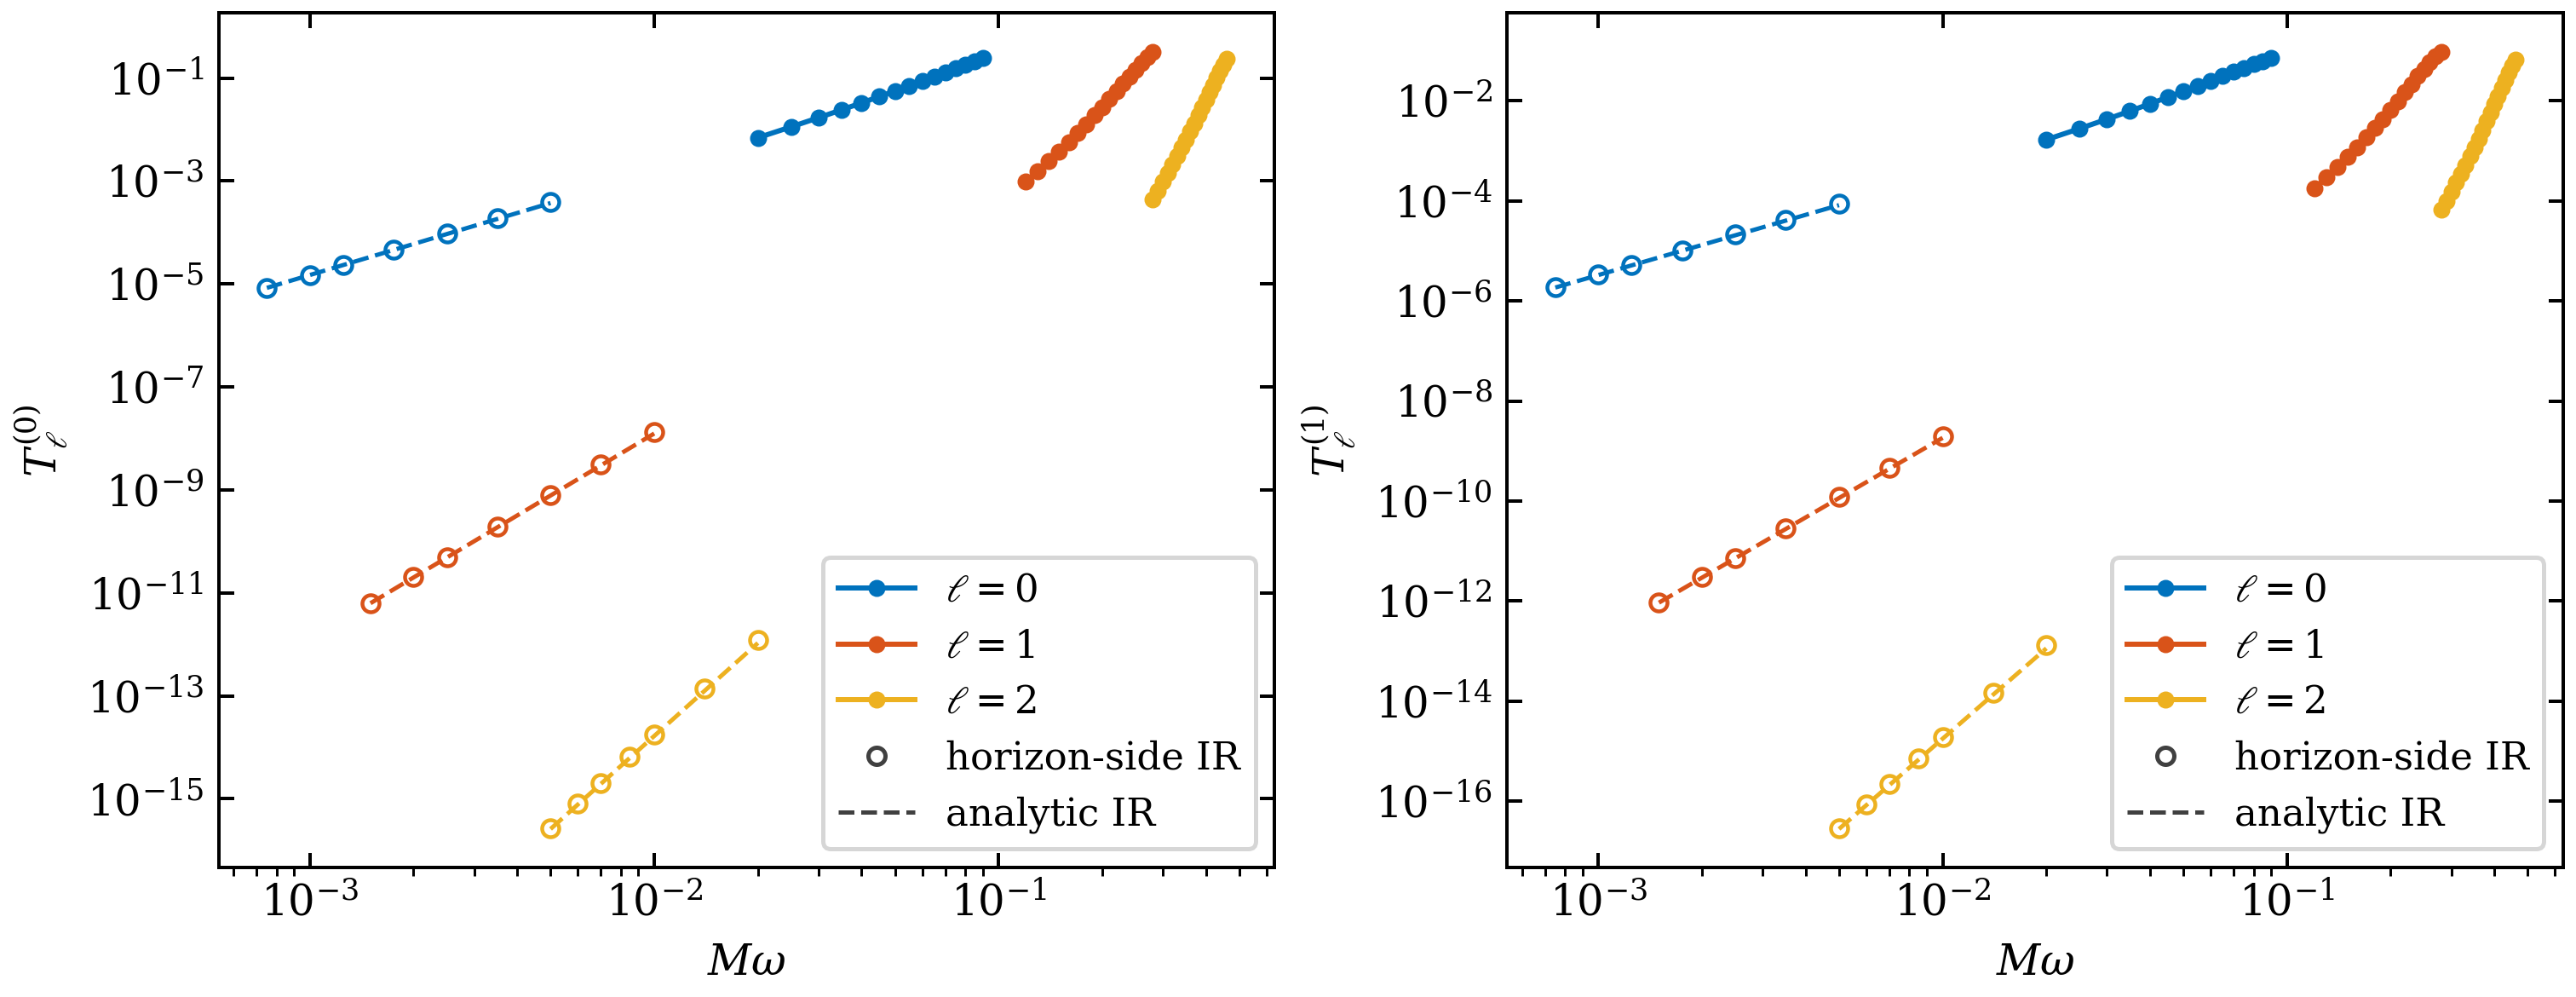
\includegraphics[width=0.92\textwidth]{kerr_scalar_low_frequency_axisymmetric.png}
\caption{Kerr 标量轴对称模的低频透射层级。图中的幂律斜率来自当前有限频窗数值拟合，用来检验不同 $\ell$ 的离心抑制层级；它们不是严格的 $\omega\to0$ 解析定理。}
\label{fig:lowfreq}
\end{figure}

\begin{table}[htbp]
\centering
\caption{$a/M=0.5$、$m=0$ 的低频有限窗拟合斜率。}
\label{tab:lowfreq-slopes}
\begin{tabular}{ccc}
\toprule
$\ell$ & $T^{(0)}$ 斜率 $\alpha_0$ & $T^{(1)}$ 斜率 $\alpha_1$ \\
\midrule
0 & 2.34386559 & 2.49618560 \\
1 & 5.25199677 & 5.47667730 \\
2 & 8.52270350 & 8.73880291 \\
\bottomrule
\end{tabular}
\end{table}

结果清楚显示随 $\ell$ 增大，线性和一阶非线性透射都受到更强的低频离心抑制。由于当前拟合窗口尚未进入任意小频率的纯渐近区，数值指数不应被等同于严格整数幂；更可靠的结论是层级顺序和随 $\ell$ 增大的抑制趋势。

\section{共振峰与有限频窗衰减}

轴对称自通道的完整频率结构见图~\ref{fig:main-results}。每个 $\ell$ 都出现势垒相关峰值。以 Lorentzian 近似峰宽 $\gamma$，并与基本准正常模频率比较，结果汇总于表~\ref{tab:resonance}。峰位接近相应 QNM 的实部，而宽度与衰减率处于同一尺度；这支持“散射势垒共振受黑洞模结构控制”的解释~\cite{Berti2009}，但不意味着非线性问题被单个 QNM 完全描述。

\begin{figure}[htbp]
\centering
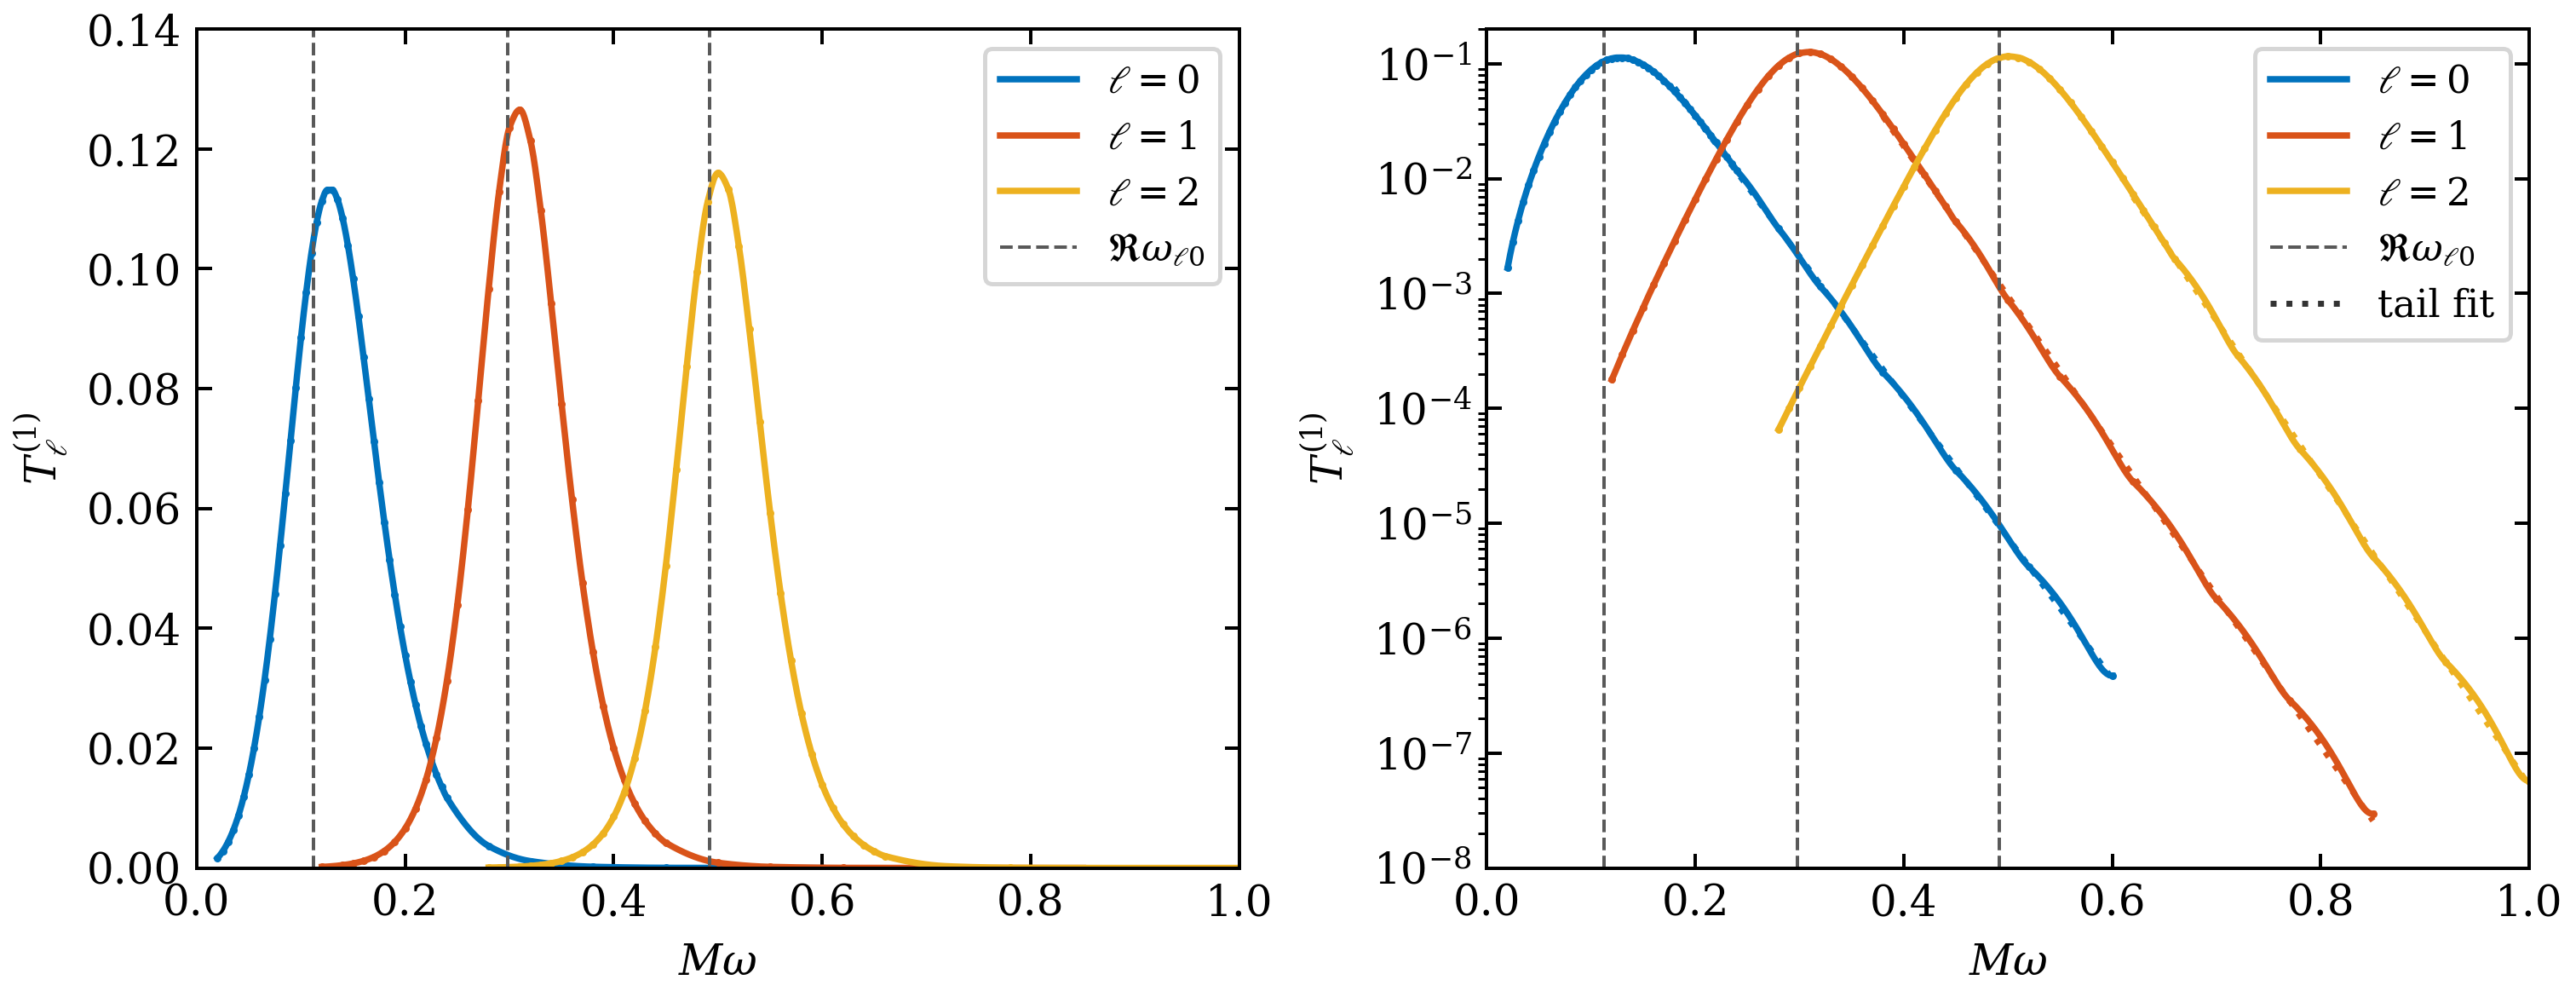
\includegraphics[width=0.96\textwidth]{kerr_scalar_nonlinear_axisymmetric_fig2.png}
\caption{Kerr $s=0$ 轴对称弱非线性散射的主要结果：线性透射、固定入射的一阶能流、共振峰以及高频有限窗口的衰减行为。所有一阶曲线均指展开系数 $T^{(1)}$，物理修正为 $\epsilon T^{(1)}$。}
\label{fig:main-results}
\end{figure}

\begin{table}[htbp]
\centering
\caption{共振拟合、QNM 对照及有限窗口指数衰减尺度。$\Delta T$ 是拟合尺度与 $\pi T_H$ 的相对差。}
\label{tab:resonance}
\begin{tabular}{cccccc}
\toprule
$\ell$ & $M\omega_{\rm peak}$ & $M\gamma$ & $M\omega_{\rm QNM}$ & $\pi MT_{\rm fit}$ & $\Delta T$ \\
\midrule
0 & 0.13057 & 0.06207 & $0.11238-0.10218\ii$ & 0.11170 & 3.73\% \\
1 & 0.31001 & 0.05974 & $0.29793-0.09536\ii$ & 0.10505 & 9.46\% \\
2 & 0.50220 & 0.06112 & $0.49196-0.09463\ii$ & 0.10151 & 12.51\% \\
\bottomrule
\end{tabular}
\end{table}

对高频有限窗口，比较
\begin{equation}
\log T^{(1)}=c-\beta M\omega,
\qquad
\log T^{(1)}=c-n\log(M\omega)
\end{equation}
两个双参数模型，指数模型相对幂律模型的 $\Delta\mathrm{AICc}$ 分别为 $48.4,31.5,17.0$；留一法交叉验证也支持指数模型。对 $a/M=0.5$，Hawking 温度
\begin{equation}
T_H=\frac{r_+-r_-}{4\pi(r_+^2+a^2)}
\end{equation}
给出 $\pi MT_H\simeq0.1160$。拟合尺度与之接近是有意义的数值线索，但现有结果只证明“在所计算的有限频率窗口内指数模型更优”，不能直接外推为严格 $\omega\to\infty$ 渐近律~\cite{Hawking1975}。

\section{数值精度、谱收敛与方程残差}

图~\ref{fig:accuracy} 汇总谱系数、离网残差、Wronskian 和能流平衡。当前全部生产点的原始径向方程离网相对残差统计为
\begin{equation}
\max\delta_R=2.8432\times10^{-10},\qquad
\delta_R^{95\%}=1.1875\times10^{-11},\qquad
\operatorname{median}\delta_R=3.1719\times10^{-13}.
\end{equation}
代表性外域和内域的 Chebyshev 尾分别约为 $2.8\times10^{-14}$ 和 $6.0\times10^{-15}$。角向活动实现与独立参考计算相比，特征值相对差不超过 $4.4\times10^{-16}$，源投影差不超过 $5.2\times10^{-14}$。

\begin{figure}[htbp]
\centering
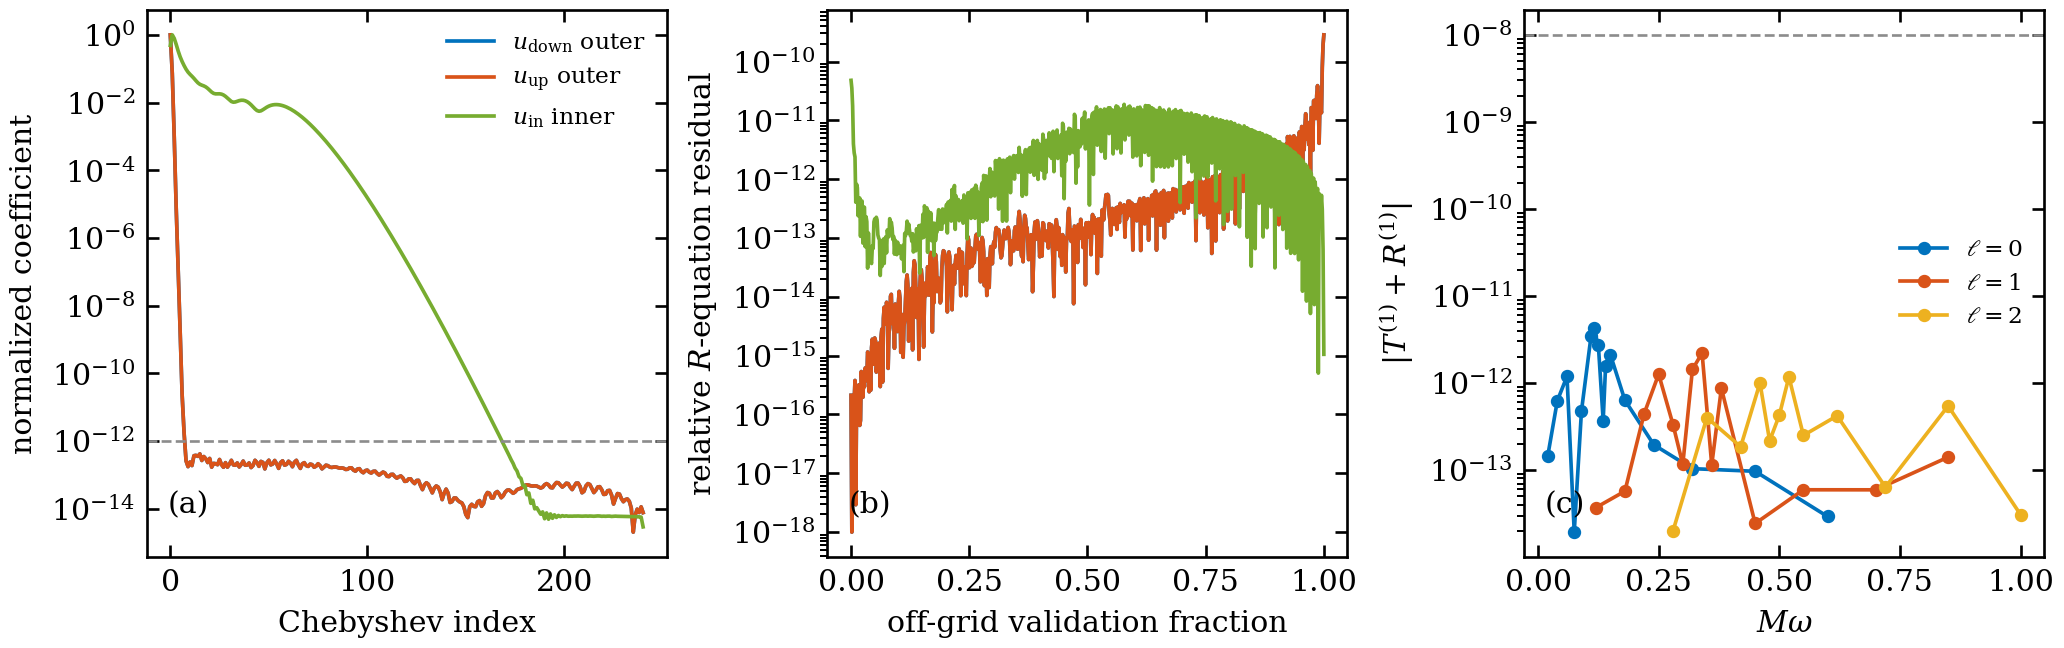
\includegraphics[width=0.96\textwidth]{kerr_scalar_axisymmetric_accuracy.png}
\caption{内部精度诊断。谱系数尾验证相位剥离未知量的解析收敛；离网残差直接验证原始 Teukolsky 方程；$\delta_0$ 和 $\delta_1$ 分别验证线性与一阶能流平衡。}
\label{fig:accuracy}
\end{figure}

这些结果说明齐次谱解已经接近双精度噪声平台。当前一阶振幅的主导误差更可能来自长程振荡 Green 积分和小量抵消，而不是径向微分方程本身。对高频代表点，远区尾阶数 $q=1792\to2048$ 引起的 $T^{(1)}$ 变化不超过 $2.5\times10^{-4}$；在固定 $q=2048$ 时降低 Chebyshev 阶数所引起的变化不超过 $9.5\times10^{-8}$。误差预算因而具有清楚的层次：
\begin{equation}
\text{齐次谱离散误差}
\ll\text{远区 Green 尾积分误差}.
\end{equation}

\section{超辐射区的一阶非线性修正}

对 $a/M=0.5$、$\ell=m=2$，阈值为
\begin{equation}
m\Omega_H=0.2679491924/M.
\end{equation}
通过一阶平衡门限的频点列于表~\ref{tab:superradiance}，图~\ref{fig:superradiance} 显示阈值两侧的符号变化。

\begin{figure}[htbp]
\centering
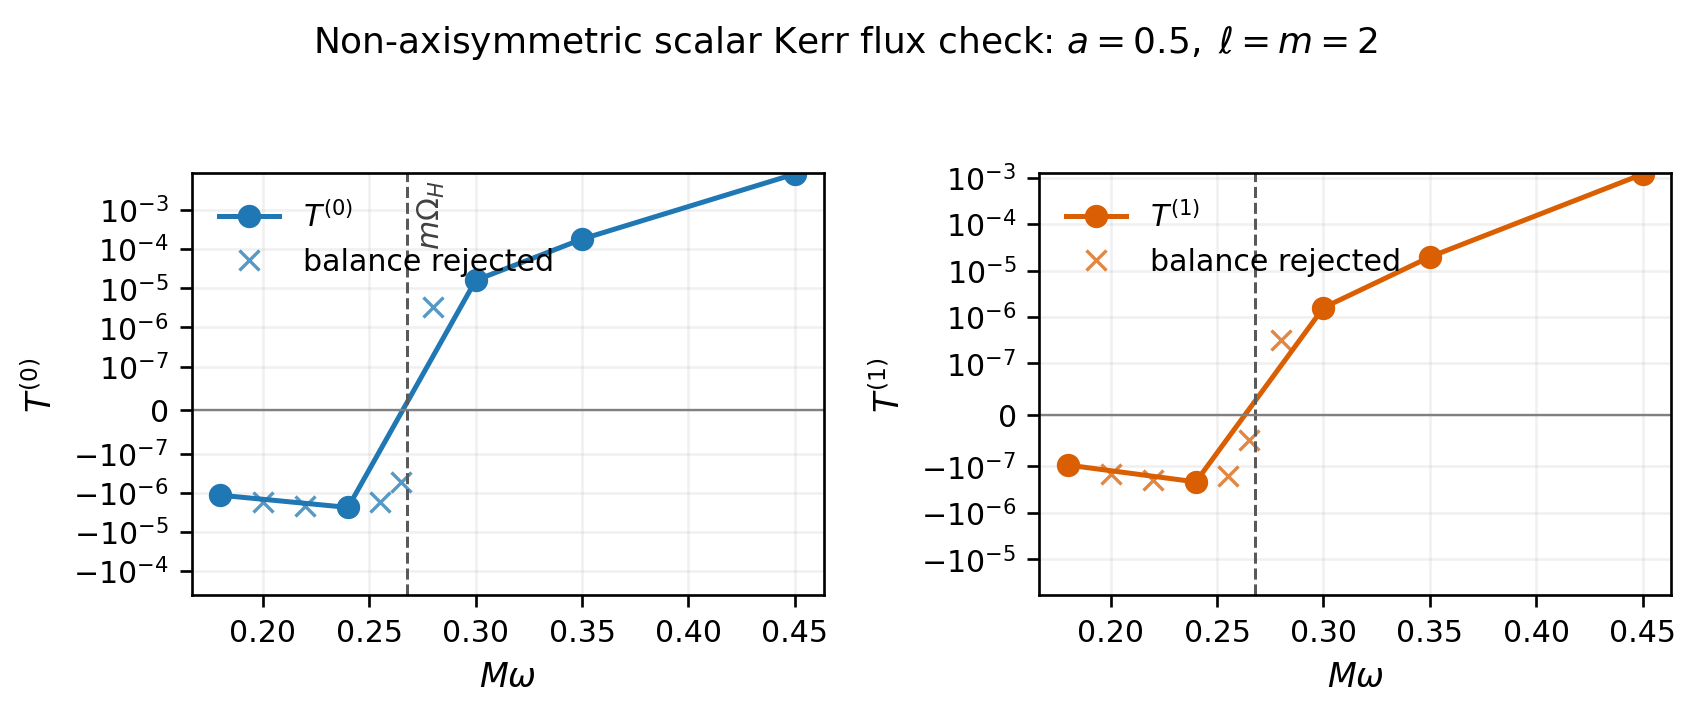
\includegraphics[width=0.93\textwidth]{kerr_scalar_nonlinear_superradiant_m2.png}
\caption{$a/M=0.5$、$\ell=m=2$ 的超辐射检验。虚线为 $M\omega=m\Omega_H$。在阈值下 $p<0$，$T^{(0)}$ 和 $T^{(1)}$ 均为负；阈值上方二者为正。}
\label{fig:superradiance}
\end{figure}

\begin{table}[htbp]
\centering
\caption{通过一阶能流平衡门限的超辐射扫描点。}
\label{tab:superradiance}
\begin{tabular}{rrrr}
\toprule
$M\omega$ & $Mp$ & $T^{(0)}$ & $T^{(1)}$ \\
\midrule
0.18 & $-0.08795$ & $-1.157\times10^{-6}$ & $-9.742\times10^{-8}$ \\
0.24 & $-0.02795$ & $-2.373\times10^{-6}$ & $-2.153\times10^{-7}$ \\
0.30 & $+0.03205$ & $+1.209\times10^{-5}$ & $+1.077\times10^{-6}$ \\
0.36 & $+0.09205$ & $+1.804\times10^{-4}$ & $+1.960\times10^{-5}$ \\
0.45 & $+0.18205$ & $+8.298\times10^{-3}$ & $+1.194\times10^{-3}$ \\
\bottomrule
\end{tabular}
\end{table}

结论不是“非线性消灭或反转超辐射”，而是：在当前微扰约定和通过平衡检查的点上，一阶修正随 $p$ 一同换号，保持超辐射能流结构。靠近阈值的若干点因 $R^{(1)}$ 中强烈的反射交叉项抵消而没有通过当前数值门限；这些点被标记为数值条件受限，不能解释成物理不连续。

\section{旋转连续性与目标通道结构}

在 $\ell=2,m=0,M\omega=0.52$ 固定时，$T^{(1)}$ 从 $a=0$ 的 $0.0894395$ 平滑上升到 $a/M=0.5$ 的 $0.103814$，且 $R^{(1)}=-T^{(1)}$。图~\ref{fig:spin-limit} 因而给出从 Schwarzschild 到 Kerr 的直接数值连续性检查。

\begin{figure}[htbp]
\centering
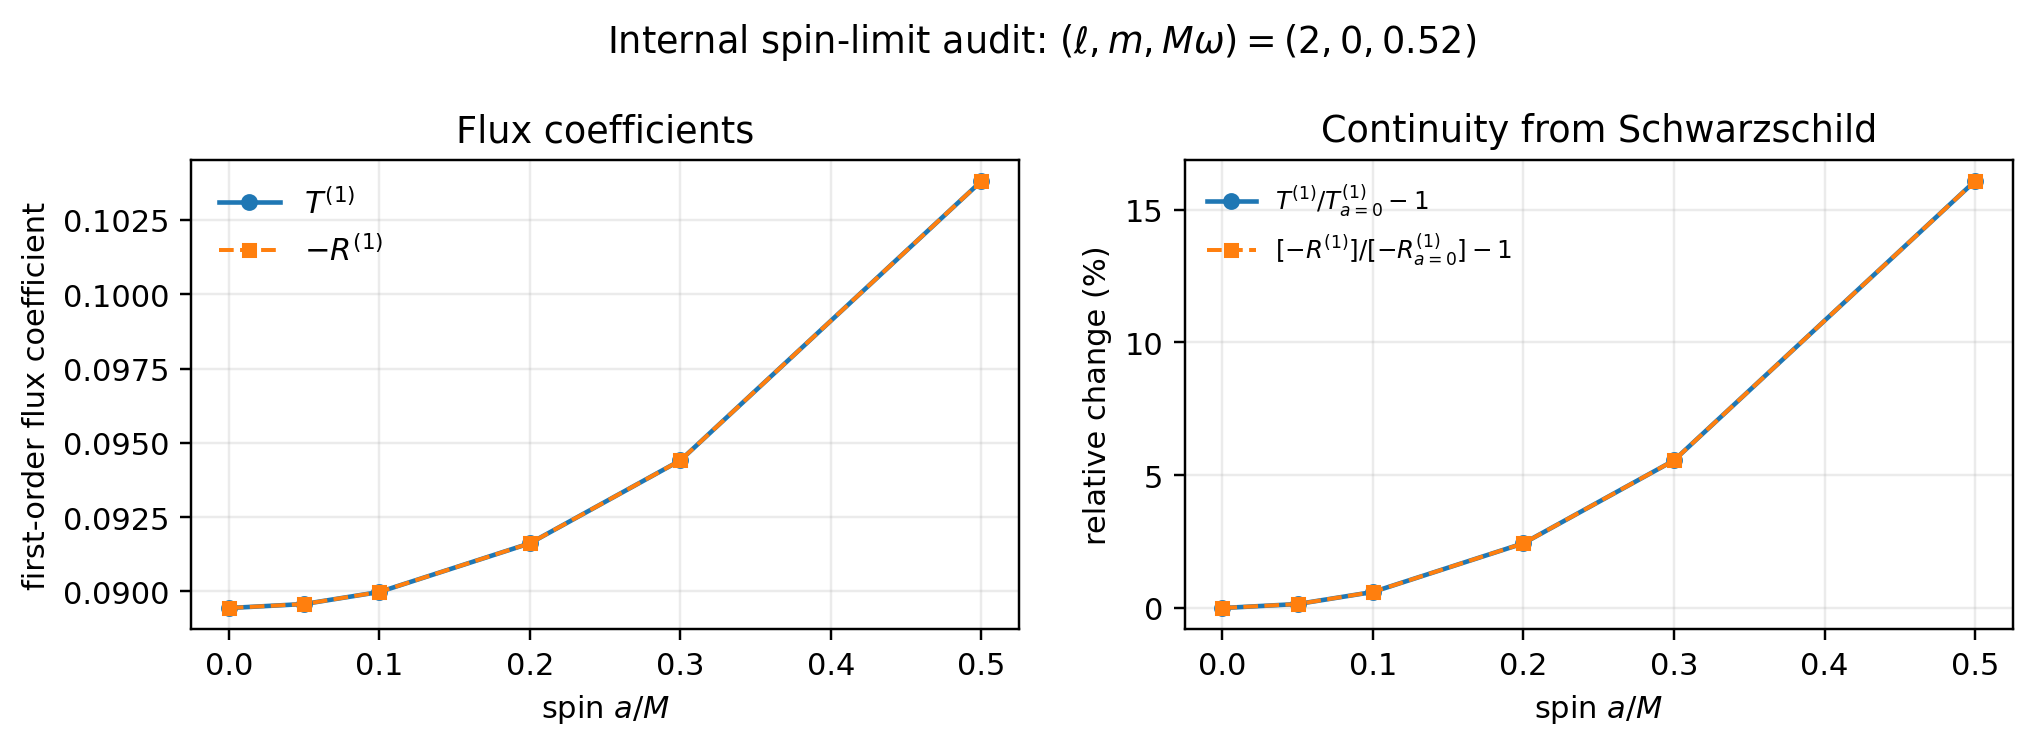
\includegraphics[width=0.93\textwidth]{kerr_scalar_spin_limit.png}
\caption{$\ell=2,m=0,M\omega=0.52$ 的旋转连续性。$T^{(1)}$ 与 $-R^{(1)}$ 重合，并从 $a=0$ 平滑延伸到 $a/M=0.5$。}
\label{fig:spin-limit}
\end{figure}

非线性源同时激发多个 $\ell'$。在 $a/M=0.5$、$\ell=m=2$、$M\omega=0.30$，代表性投影和振幅为
\begin{table}[htbp]
\centering
\caption{三次源的偶宇称目标通道。振幅为单位视界归一化的 Green 振幅，仅用于展示通道层级。}
\label{tab:channels}
\begin{tabular}{ccccc}
\toprule
$\ell'$ & $C^{(0)}$ & $C^{(2)}$ & $\abs{A_{\rm ref}^{(1)}}$ & $\abs{A_H^{(1)}}$ \\
\midrule
2 & 0.1136 & 0.01034 & $1.137\times10^6$ & $3.804\times10^3$ \\
4 & 0.03578 & 0.005513 & $1.362\times10^4$ & $1.319$ \\
6 & 0.005341 & 0.005364 & $2.265\times10^3$ & $5.383\times10^{-7}$ \\
\bottomrule
\end{tabular}
\end{table}
奇 $\ell'$ 通道由宇称严格消失。$\ell'=6$ 的视界振幅已接近条件数受限区，只能视为数量级信息。更重要的是，这些旁通道虽然在一阶场中存在，却因与零阶角向模正交，不进入总能流的 $\cO(\epsilon)$ 干涉项。

\section{项目实现路线和可复现工作流}
\label{sec:implementation}

\subsection{代码模块对应的物理层}

\begin{longtable}{>{\raggedright\arraybackslash}p{0.34\textwidth}p{0.58\textwidth}}
\caption{主要源文件与物理职责。}\label{tab:code-map}\\
\toprule
文件 & 内容 \\
\midrule
\endfirsthead
\toprule
文件 & 内容 \\
\midrule
\endhead
\path{GF_adaptive_match.m} & Schwarzschild 端点谱求解、低频映射和匹配基准。\\
\path{src/gf_adaptive_match.py} & Schwarzschild Python 实现及线性/非线性振幅计算。\\
\path{src/bondi.py} & Schwarzschild 相位剥离后方程、Chebyshev 节点和端点行。\\
\path{src/teukolsky_scalar.py} & Kerr 标量角向本征值、球状谐和径向算符定义。\\
\path{src/kerr_scalar_spectral.py} & Kerr 三分支、两域端点包含谱求解、匹配、振幅和诊断。\\
\path{src/kerr_scalar_nonlinear.py} & 三次角投影、Green 函数积分、固定入射一阶能流。\\
\bottomrule
\end{longtable}

\subsection{建议的计算顺序}

一个可靠的频点计算按下列门控顺序执行：
\begin{enumerate}
\item 求 $A_{\ell m}$，转换成式~\eqref{eq:lambda} 的 $\lambda$，检查角向归一化和本征残差；
\item 解 $R^{\rm in}$、$R^{\rm down}$、$R^{\rm up}$，检查谱尾和离网原方程残差；
\item 在 $r_m$ 解式~\eqref{eq:matching}，检查匹配条件数和 Wronskian 漂移；
\item 计算 $T^{(0)},R^{(0)}$，要求 $\delta_0$ 通过门限；
\item 计算 $C^{(0)},C^{(2)}$，检查独立角向实现；
\item 分近区和远区计算 Green 积分，对 $q$ 做收敛扫描；
\item 转换为固定入射 $T^{(1)},R^{(1)}$，要求 $\delta_1$ 通过门限；
\item 最后才把该频点纳入物理拟合、峰值分析或渐近分析。
\end{enumerate}
任何只通过某一个检查的点都不应被称为“高精度”。例如小径向残差并不能保证远区积分收敛，小 $\delta_1$ 也可能由两个错误量偶然抵消；必须联合检查式~\eqref{eq:all-diagnostics}。

\section{结论与当前边界}

从 Schwarzschild 到 Kerr，问题的核心结构保持不变：齐次散射基决定 Green 函数，三次零阶场产生一阶源，边界交叉项给出能流修正。Kerr 的新物理全部可以清楚定位：
\begin{itemize}
\item $p=\omega-m\Omega_H$ 控制视界相位、吸收符号和超辐射；
\item $S_{\ell m}(a\omega)$ 与 $\Sigma$ 权重导致 $C^{(0)}$、$C^{(2)}$ 和 $\ell'$ 混合；
\item 固定入射归一化要求三次源缩放，从而产生 $\abs{B^{\rm inc}}^4$ 分母；
\item 端点紧化后，二阶系数在真实边界消失，原方程退化为精确导数条件，不需要视界截断；
\item 自通道的局域交叉流守恒给出 $T^{(1)}+R^{(1)}=0$。
\end{itemize}

当前数值结果已经得到预期的主要物理结构：低频离心层级、势垒/QNM 相关峰、有限频窗指数型衰减偏好、超辐射阈值两侧的正确符号、以及 $a\to0$ 的平滑 Schwarzschild 极限。齐次解的谱尾和离网残差已经接近双精度精度；下一阶段若要提高高频一阶振幅，重点应放在解析远区渐近展开、相位通道求积和高精度抵消控制，而不是单纯继续增加谱阶数。

本结论严格限于固定背景、单频入射和一阶弱非线性。若 $\chi_{\rm nl}$ 不再远小于一，或者 $\abs{\epsilon}\abs{\mathcal A_{\rm in}}^2\abs{T^{(1)}}$ 与 $\abs{T^{(0)}}$ 同阶，就需要二阶微扰或时域非线性演化。本文也不包含 $s=-2$ 引力 Teukolsky 方程、黑洞自力或轨道反作用。

\appendix

\section{端点退化为何给出边界导数条件}

考虑紧区间上的一般方程
\begin{equation}
A_2(z)u''+A_1(z)u'+A_0(z)u=0.
\end{equation}
若在端点 $z=z_e$ 有 $A_2(z_e)=0$ 而 $A_1,A_0$ 有限，则对端点正则解取极限得到
\begin{equation}
A_1(z_e)u'(z_e)+A_0(z_e)u(z_e)=0.
\end{equation}
它不是额外边界条件，而是二阶方程在特征端点的降阶极限。另一个自由度由物理分支的整体归一化固定。因此数值矩阵需要两行：一行保留退化 ODE，一行施加 $u(z_e)=1$。若同时删除端点 ODE 行并只保留 Dirichlet 归一化，就丢掉了正则性；若在 $z_e-\delta$ 施加渐近条件，则引入截断误差。

\section{一阶能流系数的归一化推导摘要}

设单位视界零阶解在无穷远的入射振幅为 $I$，物理固定入射场为
\begin{equation}
\Phi_{\rm phys}^{(0)}=\frac{1}{I}\Phi_{\rm uh}^{(0)}.
\end{equation}
由于一阶算符线性、源为三次，
\begin{equation}
\Phi_{\rm phys}^{(1)}
=\frac{1}{\abs I^2I}\Phi_{\rm uh}^{(1)}.
\end{equation}
边界能流的交叉项一般为 $2\Ree[(A^{(0)})^*A^{(1)}]$。零阶边界振幅再提供一个 $1/I$ 或其共轭，故总缩放为 $1/\abs I^4$。Schwarzschild 中 $I=\widehat I$；Kerr 中 $I=\Bin$，并在视界额外保留运动学因子 $p(r_+^2+a^2)/\omega$。

\section{符号表}

\footnotesize
\begin{longtable}{p{0.31\textwidth}p{0.59\textwidth}}
\toprule
符号 & 含义 \\
\midrule
$M,a$ & 黑洞质量和单位质量角动量参数。\\
$r_\pm$ & Kerr 外/内视界半径。\\
$r_*$ & tortoise 坐标。\\
$\omega,m,\ell$ & 频率、方位量子数和角量子数。\\
$p$ & $\omega-m\Omega_H$，视界共转频率。\\
$A_{\ell m},\lambda$ & 球状谐本征值与径向 Teukolsky 分离常数。\\
$\widehat I,\widehat R$ & Schwarzschild 单位视界 in 解的无穷远入射/反射振幅。\\
$\Bin,\Bref$ & Kerr 单位视界 in 解的无穷远入射/反射振幅。\\
$A_H^{(1)},A_{\rm ref}^{(1)}$ & 单位视界约定的一阶 Green 边界振幅。\\
$T^{(0)},R^{(0)}$ & 固定入射的线性透射/反射能流系数。\\
$T^{(1)},R^{(1)}$ & 固定入射的能流一阶展开系数。\\
$\mathcal A_{\rm in}$ & 相对于单位入射约定的一般无量纲入射波幅。\\
$\epsilon\abs{\mathcal A_{\rm in}}^2T^{(1)},\epsilon\abs{\mathcal A_{\rm in}}^2R^{(1)}$ & 有限耦合和一般入射幅下的一阶物理能流修正。\\
$\eta_{\rm tail}$ & Chebyshev 谱尾指标。\\
$\delta_R,\delta_W,\delta_0,\delta_1$ & 离网方程、Wronskian、线性平衡和一阶平衡误差。\\
\bottomrule
\end{longtable}
\normalsize

\begin{thebibliography}{99}

\bibitem{Sanchez1976}
N. G. Sanchez,
``Absorption and emission spectra of a Schwarzschild black hole,''
Phys. Rev. D \textbf{18}, 1030 (1978).

\bibitem{Futterman}
J. A. H. Futterman, F. A. Handler, and R. A. Matzner,
\textit{Scattering from Black Holes}
(Cambridge University Press, Cambridge, 1988).

\bibitem{Teukolsky1973}
S. A. Teukolsky,
``Perturbations of a rotating black hole. I. Fundamental equations for gravitational, electromagnetic, and neutrino-field perturbations,''
Astrophys. J. \textbf{185}, 635 (1973).

\bibitem{StarobinskyChurilov}
A. A. Starobinsky and S. M. Churilov,
``Amplification of electromagnetic and gravitational waves scattered by a rotating black hole,''
Sov. Phys. JETP \textbf{38}, 1 (1974).

\bibitem{PressTeukolsky}
W. H. Press and S. A. Teukolsky,
``Floating orbits, superradiant scattering and the black-hole bomb,''
Nature \textbf{238}, 211 (1972).

\bibitem{MST1996}
S. Mano, H. Suzuki, and E. Takasugi,
``Analytic solutions of the Teukolsky equation and their low frequency expansions,''
Prog. Theor. Phys. \textbf{95}, 1079 (1996).

\bibitem{SasakiTagoshi}
M. Sasaki and H. Tagoshi,
``Analytic black hole perturbation approach to gravitational radiation,''
Living Rev. Relativ. \textbf{6}, 6 (2003).

\bibitem{Berti2009}
E. Berti, V. Cardoso, and A. O. Starinets,
``Quasinormal modes of black holes and black branes,''
Class. Quantum Grav. \textbf{26}, 163001 (2009).

\bibitem{Hawking1975}
S. W. Hawking,
``Particle creation by black holes,''
Commun. Math. Phys. \textbf{43}, 199 (1975).

\bibitem{GlampedakisAndersson2001}
K. Glampedakis and N. Andersson,
``Scattering of scalar waves by rotating black holes,''
Class. Quantum Grav. \textbf{18}, 1939 (2001).

\bibitem{Dafermos2018}
M. Dafermos, G. Holzegel, and I. Rodnianski,
``Boundedness and decay for the Teukolsky equation on Kerr spacetimes I: The case $|a|\ll M$,''
Ann. PDE \textbf{5}, 2 (2019).

\bibitem{Stein2019}
L. C. Stein,
``qnm: A Python package for calculating Kerr quasinormal modes, separation constants, and spherical-spheroidal mixing coefficients,''
J. Open Source Softw. \textbf{4}, 1683 (2019).

\end{thebibliography}

\end{document}
